\documentclass[letterpaper,12pt,]{article}

\usepackage[%
    left=1in,%
    right=1in,%
    top=1in,%
    bottom=1.0in,%
    paperheight=11in,%
    paperwidth=8.5in%
]{geometry}%

\usepackage{listings}
\usepackage{graphicx}
\usepackage{amsmath}
\usepackage[font=small,skip=-2pt]{caption}
\usepackage{subcaption}
\usepackage{hyperref}
\usepackage{booktabs}
\usepackage{pdfpages}
\usepackage{pgffor}
\usepackage[section]{placeins}


\lstdefinestyle{mystyle}{
    %backgroundcolor=\color{backcolour},
    %commentstyle=\color{codegreen},
    %keywordstyle=\color{magenta},
    %numberstyle=\tiny\color{codegray},
    %stringstyle=\color{codepurple},
    basicstyle=\footnotesize,
    breakatwhitespace=false,
    breaklines=true,
    captionpos=b,
    keepspaces=true,
    numbers=left,
    numberstyle=\footnotesize,
    stepnumber=1,
    numbersep=5pt,
    showspaces=false,
    showstringspaces=false,
    showtabs=false,
    tabsize=2,
    frame=single
}
\lstset{frame=single}

\pagestyle{empty} % Remove page numbering
\linespread{1.5} % Line Spacing

\begin{document}

\begin{titlepage}

\newcommand{\HRule}{\rule{\linewidth}{0.5mm}} % Defines a new command for the horizontal lines, change thickness here

\center % Center everything on the page
 
%----------------------------------------------------------------------------------------
%	HEADING SECTIONS
%----------------------------------------------------------------------------------------


\textsc{\LARGE McGill University}\\[3.5cm]
\textsc{\Large Computational Aerodynamics}\\[0.5cm] 
\textsc{\large MECH 539}\\[2.5cm]

%----------------------------------------------------------------------------------------
%	TITLE SECTION
%----------------------------------------------------------------------------------------

{ \huge \bfseries Project 2}\\[1.5cm] % Title of your document

\HRule \\[0.4cm]
%----------------------------------------------------------------------------------------
%	AUTHOR SECTION
%----------------------------------------------------------------------------------------

\begin{minipage}{0.4\textwidth}
\begin{flushleft} \large
\emph{Name:}\\
Doug \textsc{Shi-Dong} % Your name
\end{flushleft}
\end{minipage}
~
\begin{minipage}{0.4\textwidth}
\begin{flushright} \large
\emph{Student ID:} \\
260466662\\
\end{flushright}
\end{minipage}\\[4cm]

\vfill{}
{\large February 18, 2016}\\[2cm]

\end{titlepage}


\section*{Question 1}

\begin{figure}[!ht]
    \centering
    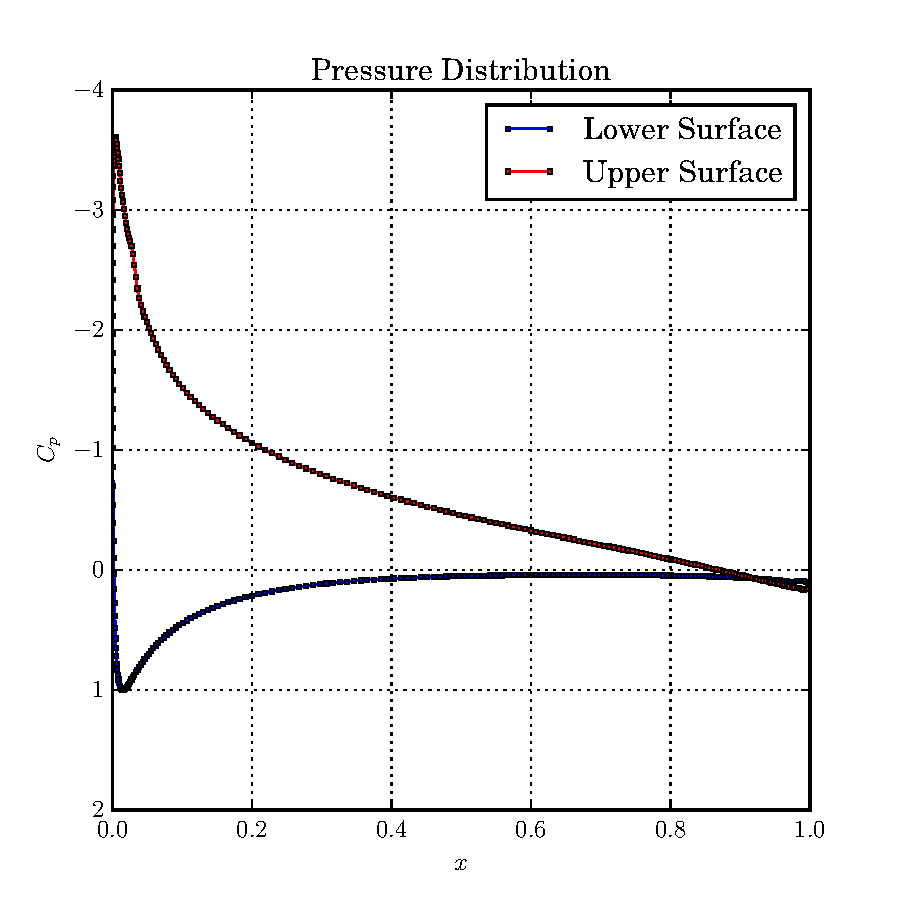
\includegraphics[width = 0.85\textwidth]{./Figures/q1.pdf}
    \caption {Surface Pressure Distribution}
    \label{fig:q1}
\end{figure}

Figure \ref{fig:q1} shows the pressure distribution on the lower and upper surface of the airfoil.
Most of the pressure difference occurs at the leading edge, where the flow is accelerated on the upper surface and decelerated on the lower surface.

Afterwards, flow is decelerated on the upper surface due to the adverse pressure gradient.
Near the leading edge of the upper surface, a small drop in suction occurs.
This can be explained by the formation of a recirculation bubble due to adverse pressure gradient.
This will in effect cause the transition from laminar to turbulent flow.

There is also turbulent separation near the trailing edge of the upper surface.
It is barely noticeable on the pressure distribution plot, but it will be more apparent in Section 2, when the skin friction coefficient is investigated.

The flow on the lower surface is accelerated due to a favorable pressure gradient. In effect, the transition from laminar to turbulent from doesn't occur until near the trailing edge.

\section*{Question 2}

\begin{figure}[!ht]
    \centering
    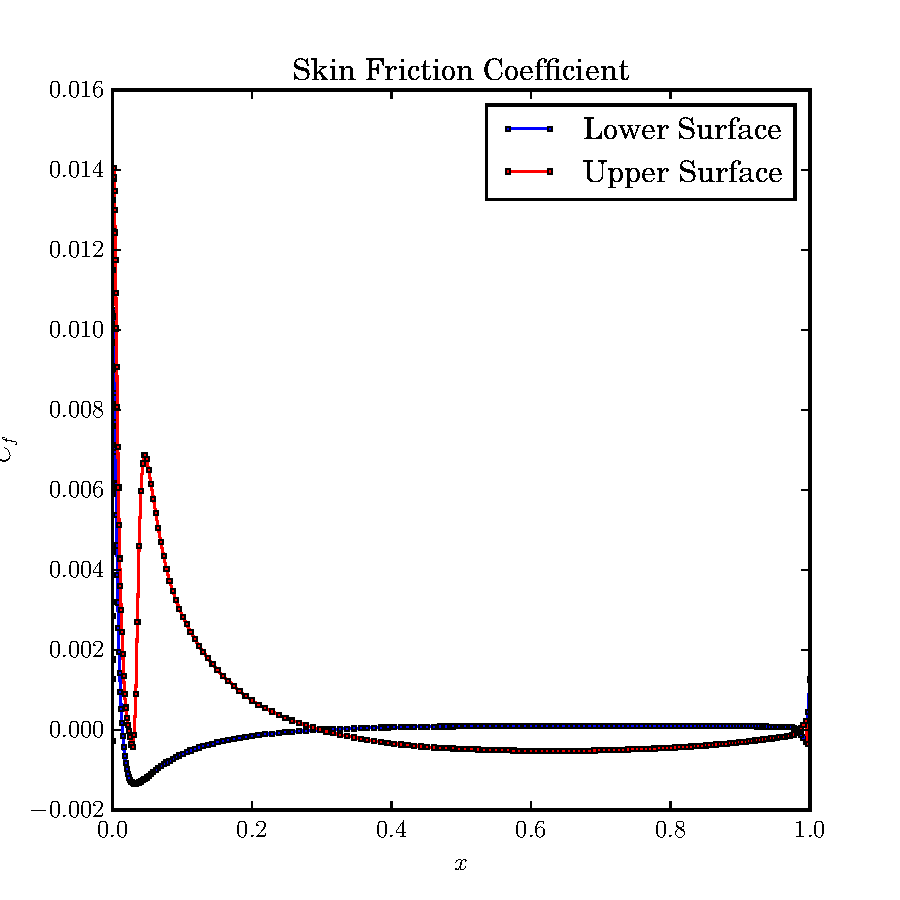
\includegraphics[width = 0.85\textwidth]{./Figures/q2.pdf}
    \caption {Skin Friction Coefficient Distribution}
    \label{fig:q2}
\end{figure}

Figure \ref{fig:q2} shows the skin friction coefficient ($C_f$) distribution over the airfoil.
Note that the tangent direction of the surface is taken with respect to the stagnation point, such that a negative $C_f$ points upstream.

The upper surface shows two regions where the skin friction coefficient becomes negative, whereas the lower region shows one region near the trailing edge.
Since the velocity gradient is negative and the velocity at the wall is 0, there must be flow reversal in those regions of negative $C_f$.
Flow reversal signifies the presence of a re-circulation bubble.

The upper surface laminar separation is quickly followed by turbulent re-attachment.
This results in a significant increase in the skin friction coefficient, since turbulent flows have a greater velocity gradient.

Since the lower surface stays laminar for the most part, the $C_f$ is smaller than for the upper surface. In fact, most of the viscous drag is created from the upper surface.



\section*{Question 3}
\begin{table}[!h]
\centering
\begin{tabular}{ccccccc} \toprule
    {} & {$C_L$} & {$C_D$} &
         {$C_{L_{exp}}$\cite{ladson}} & {$C_{D_{exp}}$\cite{ladson}} &
         {$C_{L_{exp}}$\cite{greg}} & {$C_{D_{exp}}$\cite{greg}}\\
         \midrule
    {Pressure}  &  0.80906  & 0.004845 &&&&\\
    {Viscous}   & -0.00009  & 0.004942 &&&&\\
    {Total}     &  0.80897  & 0.009787 & $0.808970^*$ & $0.011899^*$ &$0.8^{**}$&$0.011^{**}$\\
\bottomrule
\end{tabular}
\vspace{-0.5em}
\begin{flushleft}
{\tiny 
\hspace{5em}* Interpolated Data, ** Visually extracted from figure}
\end{flushleft}
\caption{Lift and Drag Coefficients of NACA0012}
\label{tab1}
\end{table}

Table \ref{tab1} shows the lift and drag coefficients computed from the numerical results and the experimental results.
The experimental data comes from Ladson\cite{ladson} and Gregory \& O'Reilly\cite{greg}.

Viscosity has a negligible effect on lift, but contributes almost equally to drag. At a Reynolds number of 2 million, this is expected.

The numerical results seem to underestimate the drag coefficient compared to both sources of experimental data.
This could be due to the fact that the numerical simulation is done on a 2D airfoil.
First, induced drag is not taken in account since it requires a finite wing span.
Second, turbulence which is inherently three-dimensional may not be modeled accurately.
Since the flow solver method and parameters, it is hard to critique the accuracy of the solution.
Note that experimental error is also present.

\section*{Question 4 \& 5}

Figure \ref{fig:q4air} shows the different flow regimes on the airfoil. The lower surface is almost entirely laminar, while the upper surface is almost entirely turbulent. Re-circulation bubbles regions are also shown before the flow re-attaches.

Laminar separation occurs at the leading edge of the upper surface and the trailing edge of the lower surface as mentioned in Question 2.
Turbulent separation only occurs at the trailing edge of the upper surface.

\begin{figure}[!h]
    \centering
    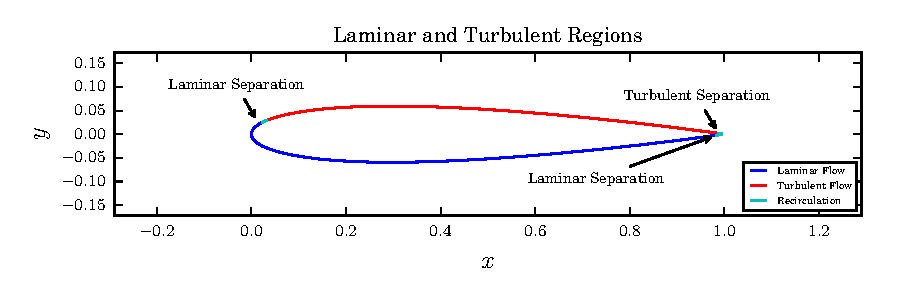
\includegraphics[width = 1.0\textwidth]{./Figures/q4airfoil.pdf}
    \caption {Flow Behavior along the Surface}
    \label{fig:q4air}
\end{figure}

Figure \ref{fig:q5lam} \& \ref{fig:q5turb} show laminar and turbulent $u^+$ versus $y^+$ plots at $x=0.5$ on the lower and upper surface respectively.
The velocity profile in the laminar region closely follows the linear relationship between $u^+$ and $y^+$.
Since the boundary layer is laminar, the shear from viscous effects dominates, therefore the turbulent log-law does not apply.

The velocity profile of the turbulent region shows that the viscous sublayer extends up to approximately $y^+=3$.
In the log-law region, the numerical result is offset and the slope is off from the analytical approximation. However, a log-law trend is present in the numerical solution.


\begin{figure}
    \centering
    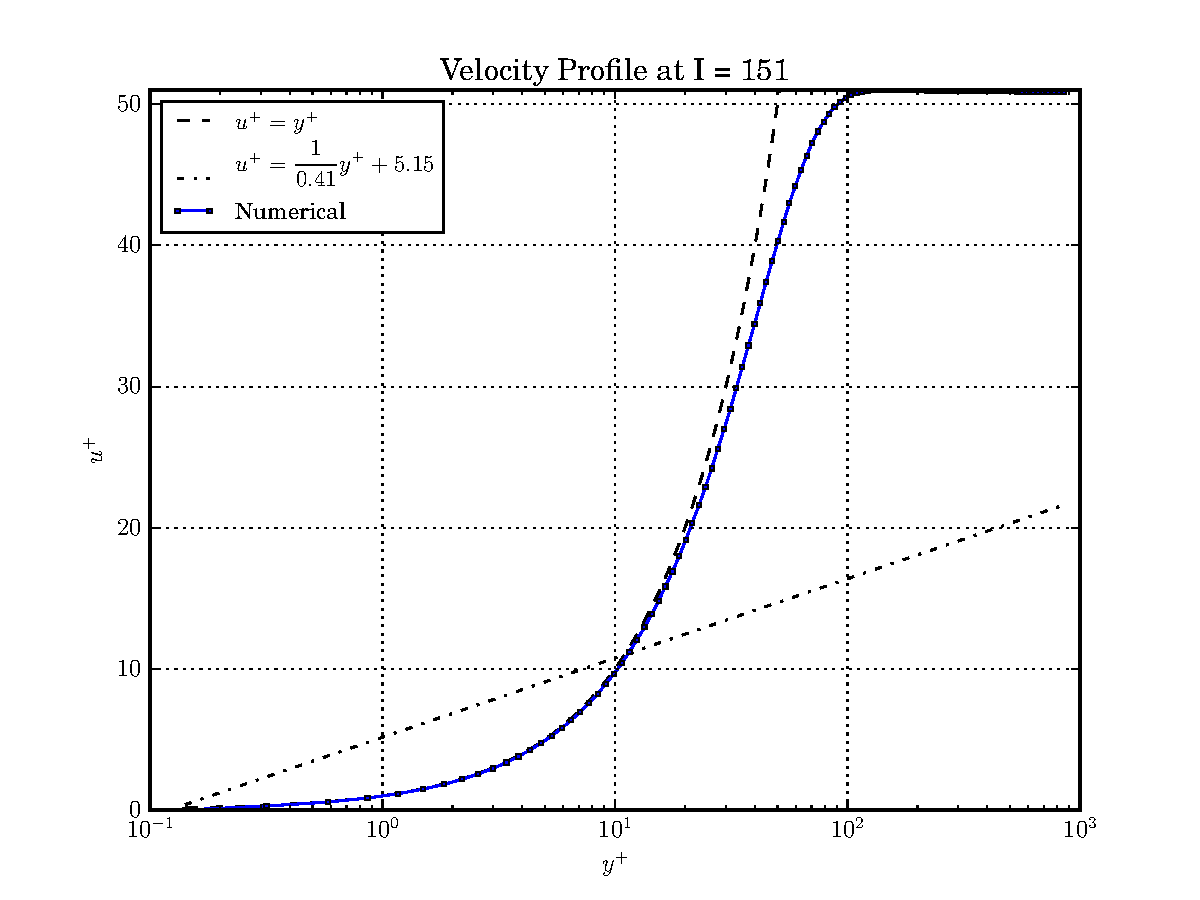
\includegraphics[width = 0.85\textwidth]{./Figures/q5lam.pdf}
    \caption {Laminar Velocity Profile on Lower Surface at $x=0.5$}
    \label{fig:q5lam}
\end{figure}

\begin{figure}
    \centering
    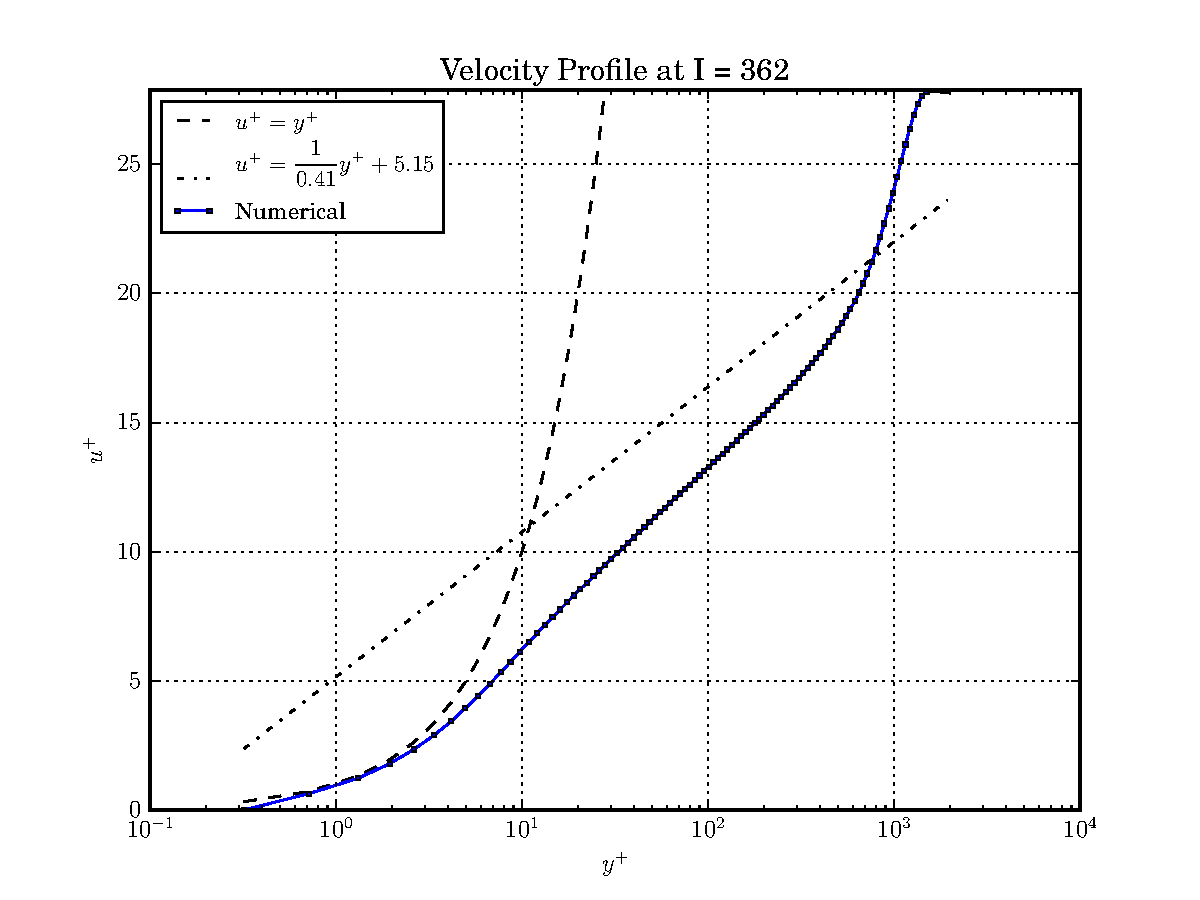
\includegraphics[width = 0.85\textwidth]{./Figures/q5turb.pdf}
    \caption {Turbulent Velocity Profile on Upper Surface at $x=0.5$}
    \label{fig:q5turb}
\end{figure}


\section*{Question 6}
\begin{figure}[!h]
    \centering
    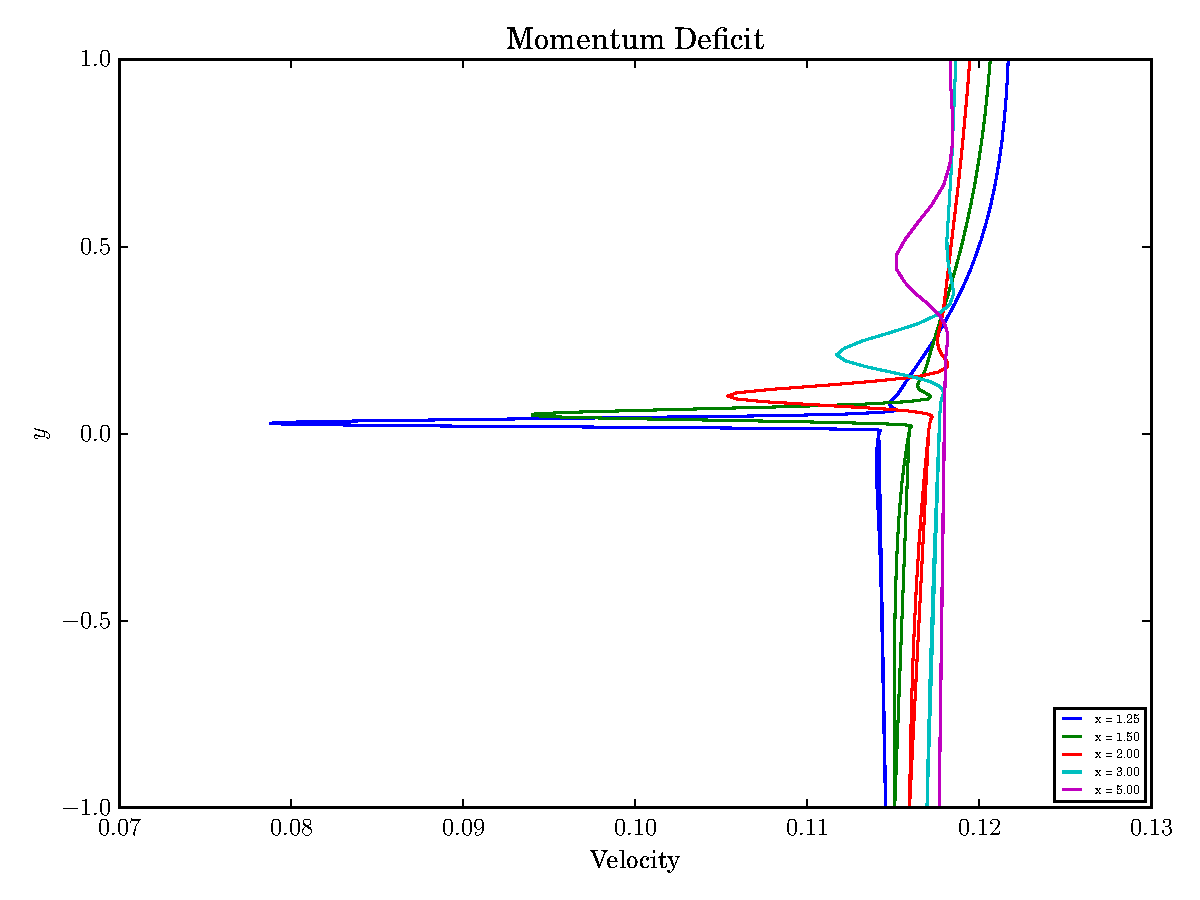
\includegraphics[width = 0.8\textwidth]{./Figures/q6.pdf}
    \caption {Momentum Profiles at Different $x$-locations}
    \label{fig:q6}
\end{figure}

Figure \ref{fig:q6} shows a slice of the velocity at different $x$-locations.
The values are interpolated such that $x$ stays constant.
A momentum deficit can clearly be seen in the wake.
This momentum deficit is caused by the convection of the boundary layer.

Closer to the airfoil, there is a large thin momentum deficit.
This momentum deficit gets convected downstream.
As it gets convected, the deficit moves in the $y$-direction and diffuses into a wider lower-magnitude.
It gets convected because of the angle of attack of the incoming flow and diffuses since it has to respect the boundary condition when it reaches the farfield.

The momentum deficit is closely related to the viscous drag.
Looking at the momentum equation of the Navier-Stokes, we can see that the dissipation of momentum originates from the shear stress term.
Therefore, momentum that has been lost was used to create shear stress on the wall.

\section*{Code}

Post-processing code has been written in Python available on my Github

\url{https://github.com/dougshidong/mech539/tree/master/a5}

\begin{thebibliography}{1}

\bibitem{ladson} C.L. Ladson, {\em Effects of Independent Variation of Mach and Reynolds Numbers on the Low-Speed Aerodynamic Characteristics of the NACA0012 Airfoil Section}, NASA TM 4074, 1988

\bibitem{greg} N. Gregory \& C.L. O'Reilly, {\em Low-Speed Aerodynamic Characteristics of NACA 0012 Aerofoil Section, including the Effects of Upper-Surface Roughness Simulating Hoar Frost}, NASA R\&M 3726, 1973

\end{thebibliography}
\end{document}
